
\section{Schemat Logiczny Podłączenia Internetu Mobilnego}

    \subsection{Schemat Ogólny}
    Poniższy schemat przedstawia ogólny sposób podłączenia internetu mobilnego do operatora Plus:

    \begin{figure}[!htb]
        \centering
        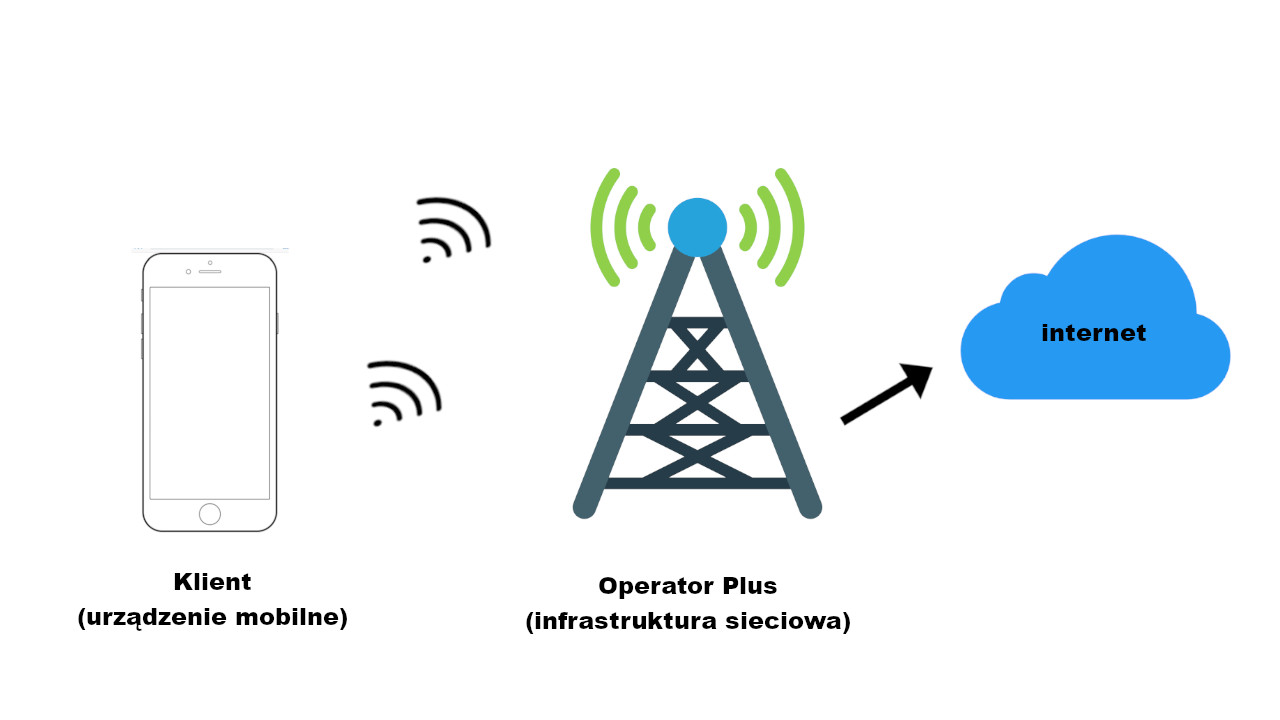
\includegraphics[width=0.8\textwidth]{schemat}
        \caption{Klient(Urządzenie mobilne)--> Operator Plus (Infrastruktura sieciowa operatora)--> Internet}
    \end{figure}



    \subsection{Połączenie z Internetem}

    Aby korzystać z usługi internetu mobilnego operatora Plus, klient musi zainicjować połączenie z siecią operatora. Proces ten wygląda następująco:
    
    \begin{enumerate}
        \item \textbf{Urządzenie Mobilne}: Klient korzysta z urządzenia mobilnego, takiego jak smartfon, tablet lub modem, które jest kompatybilne z siecią Plus. To urządzenie jest wyposażone w moduł komunikacji bezprzewodowej, który umożliwia połączenie z siecią komórkową operatora.
    
        \item \textbf{Karta SIM}: W urządzeniu klienta znajduje się karta SIM od operatora Plus. Karta SIM jest niezbędna do identyfikacji klienta w sieci i umożliwia dostęp do usług operatora.
    
        \item \textbf{Wybór Sieci}: Urządzenie mobilne klienta automatycznie wykrywa dostępne sieci operatora Plus oraz inne dostępne sieci w zasięgu. Klient wybiera sieć operatora Plus jako preferowaną sieć.
    
        \item \textbf{Nawiązanie Połączenia}: Po wybraniu sieci operatora Plus, urządzenie mobilne nawiązuje połączenie z bazową stacją operatora. To połączenie jest kluczowe do uzyskania dostępu do usług internetu.
    
        \item \textbf{Żądania i Odpowiedzi}: Klient używa swojego urządzenia mobilnego do przesyłania żądań do Internetu. Żądania te mogą obejmować przeglądanie stron internetowych, wysyłanie wiadomości e-mail, strumieniowanie treści multimedialnych i wiele innych. Sieć operatora Plus przekazuje te żądania do Internetu i przesyła odpowiedzi zwrotne z Internetu z powrotem do urządzenia klienta.
    
        \item \textbf{Szyfrowanie Danych}: W celu zapewnienia prywatności i bezpieczeństwa klienta, wiele z tych transmisji jest zabezpieczonych za pomocą odpowiednich protokołów szyfrowania, takich jak SSL/TLS (Secure Sockets Layer/Transport Layer Security) w przypadku przeglądania stron internetowych.
    
        \item \textbf{Kontrola Ruchu Danych}: Operator Plus kontroluje ruch danych klienta, w tym ilość przesyłanych danych, prędkość transmisji i inne parametry, które mogą wpływać na jakość usługi.
    
        \item \textbf{Odbiór Odpowiedzi}: Odpowiedzi zwrotne z Internetu są wyświetlane na urządzeniu klienta, umożliwiając klientowi korzystanie z różnych usług i treści dostępnych w sieci.
    
    \end{enumerate}
    
    To podstawowy proces, który opisuje, jak klient korzysta z usługi internetu mobilnego operatora Plus. Proces ten odbywa się w czasie rzeczywistym, umożliwiając klientowi szybki i niezawodny dostęp do zasobów internetu.
    
    

\pagebreak